%%%%%%%%%%%%%%%%%%%
% razor variables
%%%%%%%%%%%%%%%%%%%

% add full derivation
% plots of signal and background

Many extensions of the Standard Model (see chapter~\ref{chap:beyond_standard_model}) predict the 
existence of new particles, which can be pair-produced in the proton-proton collisions at the LHC. 
Some of those theories introduce an extra symmetry, such as the R-parity in supersymmetry. A
consequence of this symmetry is that the lightest BSM particle must be stable, as it cannot decay
to SM particles only. This lightest BSM particle, called LSP in supersymmetric theories, is weakly
interacting, and escapes the detector unseen. 

This general property leads to a generic class of new physics signatures in which a heavy
particle is pair-produced, and decays into visible, i.e. interacting with detector material, SM
particles, and an invisible LSP. This signature is illustrated in figure~\ref{fig:razor_signature}.

\begin{figure}[htb]
  \centering
  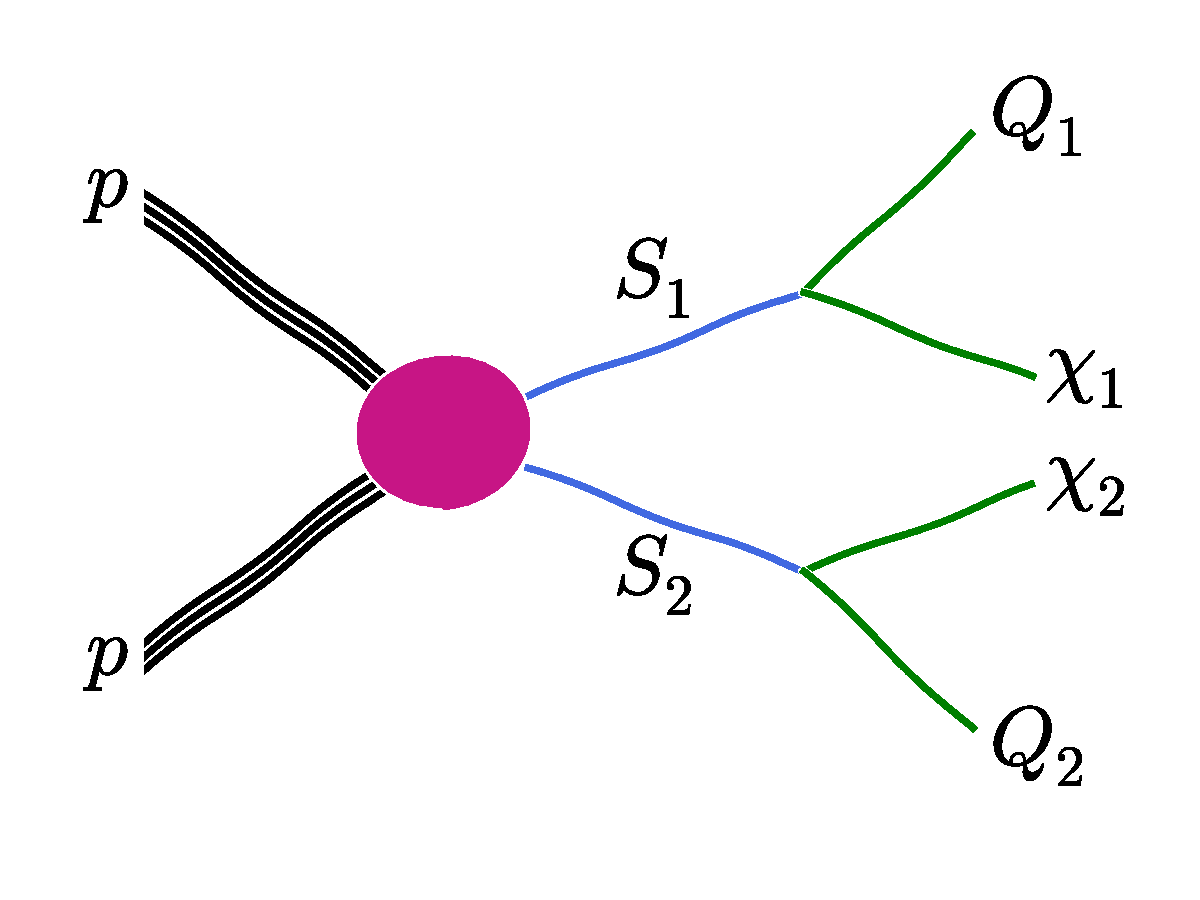
\includegraphics[width=0.6\textwidth,clip=true,trim=0 1.8cm 0
0.8cm]{figures/razor_variables/signature} 
  \caption{Generic new physics signature. Two massive new particles, $S_1$ and $S_2$, are produced
in $\Pp\Pp$ collisions at the LHC, and consequently decay to a visible system $Q_i$ and an invisible
system $\chi_i$. \label{fig:razor_signature}}
\end{figure}

Several kinematical variables targetting this topology have been
developed~\cite{Lester:1999tx,Barr:2003rg,Randall:2008rw,Polesello:2009rn,Bai:2012gs}.
% TODO add citations here
Most of these variables rely on the presence of the invisible LSP's. This causes the visible system
to deviate from a di-jet topology, resulting in possibly large missing transverse momentum, altered
angular distributions, et cetera. All of this can be used to distinguish the sought-after signal
from the known background processes. 
Unfortunately, the ultimate goal of reconstructing the masses of the new particles cannot be
attained. Because of the escaping LSP's, there is simply not enough information available to fully
constrain the problem. What we can do, however, is approximate the mass scale of the new physics
particles. Often times this results in variables that exhibit a kinematic edge. 
The \textit{razor variables} \cite{rogan,Rogan:1557072,Chatrchyan:2011ek,Chatrchyan:2014goa} are no
exception in this regard. One advantage the razor variables have over many other variables, is that
they also reconstruct the mass scale as a peak, in addition to a kinematic edge. 
In what follows I will derive the two razor variables, denoted \mr and \rsq, which use longitudinal
and transverse event information, respectively, to estimate a characteristic mass scale associated
with the new particles. At the end of this section I will briefly show how the razor variables are
used in the razor boost analysis. 

% explain reference frames

\subsection{Kinematical configuration and notation \label{sec:razor_notation}}

Let's again consider figure~\ref{fig:razor_signature}. For simplicity, we will assume that the
produced particles $S_1$ and $S_2$ undergo a two-body decay. Each $S_i$ decays to a visible,
standard model particle $Q_i$, and a particle $\chi_i$ that escapes the detector. 
We assume a symmetric decay chain, with the following relations for the masses of the different
particles,
\begin{alignat}{3}
  M_{S_1} &= M_{S_2} &&= M_S \label{eq:equal_S_masses}\\
  M_{\chi_1} &= M_{\chi_2} &&= M_{\chi} \label{eq:equal_chi_masses}\\
  M_{Q_1} &= M_{Q_2} &&= 0 \label{eq:no_Q_masses}
\end{alignat}

There are four relevant reference frames for our goal of determining a characteristic mass scale
of the new physics process under consideration. The following paragraphs will go through each of
these and define the notations that will be used, as well as deriving relations between several
variables. 

\paragraph{$S_1$ rest frame} 
From basic two-body decay kinematics it follows that the $Q_1$ and $\chi_1$ particles are produced
back to back, with equal magnitude of momentum, in the rest frame of the $S_1$ particle. This is
illustrated in figure~\ref{fig:razor_S1_rest_frame}. 

\begin{figure}[htpb]
  \centering
  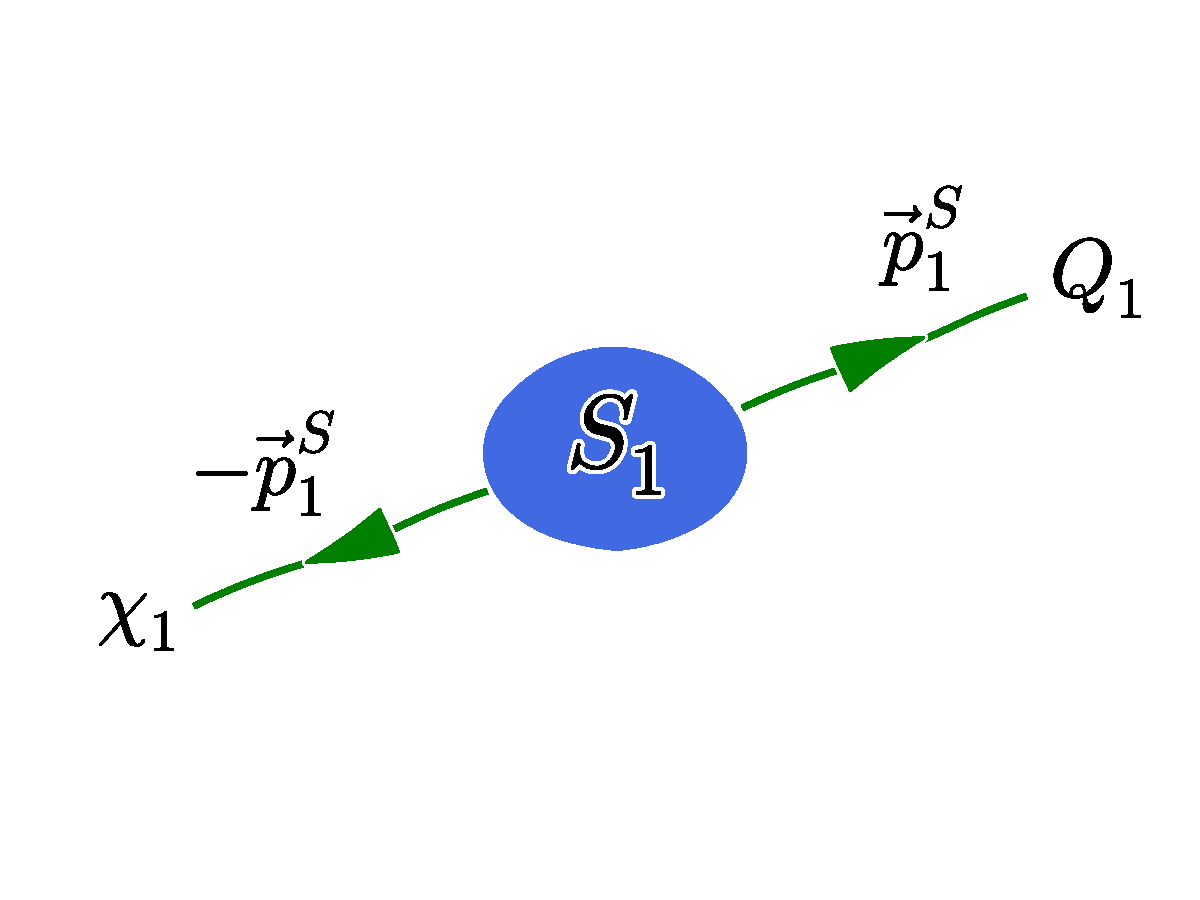
\includegraphics[width=0.6\textwidth,clip=true,trim=0 4cm 0
3cm]{figures/razor_variables/rest_frame}
  \caption{Configuration of the $S_1$ rest frame. The decay products $Q_1$ and $\chi_1$ are
produced back to back with momenta $\vec{p}^{\,S}_1$ and $-\vec{p}^{\,S}_1$, respectively. 
\label{fig:razor_S1_rest_frame}}
\end{figure}

We can compute the magnitude of this momentum in terms of the new particle masses. To do this we
start from the four-vectors $P$ of the $Q_1$ and $\chi_1$ particles in the $S_1$ rest frame, 
\begin{alignat}{6}
  P[Q_1]    &\equiv q_1^S   &&= \{ E^S_{Q_1}, \vec{q}^{\,S}_1\} , \\
  P[\chi_1] &\equiv \nu_1^S &&= \{ E^S_{\chi_1}, \vec{\nu}^{\,S}_1\} .
\end{alignat}
Conservation of energy in the $S_1$ rest frame leads to 
\begin{equation}
  E^S_{Q_1} + E^S_{\chi_1} = M_S . \label{eq:razor_conservation_energy}
\end{equation}
This can also be expressed as
\begin{equation}
  \sqrt{M_{Q_1}^2 + (\vec{q}^{\,S}_1)^2 } + \sqrt{M_{\chi_1}^2 + (\vec{\nu}^{\,S}_1)^2} = M_S .
\end{equation}
Using Eq.~\ref{eq:equal_chi_masses}, Eq.~\ref{eq:no_Q_masses} (massless $Q_1$), and the equal
momenta $|\vec{q}^{\,S}_1| = |\vec{\nu}^{\,S}_1| = |\vec{p}^{\,S}_1|$, the above can be simplified
as
\begin{align}
  |\vec{p}^{\,S}_1|   &= M_S - \sqrt{M_{\chi}^2 + (\vec{p}^{\,S}_1)^2} \\
  (\vec{p}^{\,S}_1)^2 &= M_S^2 - 2 M_S \sqrt{M_{\chi}^2 + (\vec{p}^{\,S}_1)^2} + M_{\chi}^2 +
(\vec{p}^{\,S}_1)^2 \\
  2 M_S \sqrt{M_{\chi}^2 + (\vec{p}^{\,S}_1)^2} &= M_S^2 + M_{\chi}^2 \\
  4 M_S^2 (\vec{p}^{\,S}_1)^2 &= (M_S^2)^2 + 2 M_S^2 M_{\chi}^2 + (M_{\chi}^2)^2 - 4 M_S^2
M_{\chi}^2 \\
  (\vec{p}^{\,S}_1)^2 &= \frac{(M_S^2 -M_{\chi}^2 )^2}{4 M_S^2} .
\end{align}

We thus find for the magnitude of the momentum of $Q_1$ and $\chi_1$ in the $S_1$ rest frame
\begin{equation}
  |\vec{p}^{\,S}_1| = \frac{M_S^2 -M_{\chi}^2}{2 M_S} \equiv \frac{M_\Delta}{2} ,
\label{eq:razor_p_S1_rest_frame}
\end{equation}
where we have defined the characteristic scale $M_\Delta$. This scale is exactly the scale we are
interested in. The goal of the \textbf{razor variables} is to \textbf{express $M_\Delta$ using lab
frame quantities only}. To succeed in this effort, we need to make several, physics-motivated,
approximations. These will remove the unknown degrees of freedom, and are further explained in
sections~\ref{sec:razor_mr} and \ref{sec:razor_r2}. 

The energy of the $Q_1$ and $\chi_1$ particles can also be computed easily. 
From the masslessness of $Q_1$, we immediately find using Eq.~\ref{eq:razor_p_S1_rest_frame}
\begin{equation}
  E^S_{Q_1} = |\vec{p}^{\,S}_1| = \frac{M_\Delta}{2}. \label{eq:razor_E_Q1}
\end{equation}
To compute $E^S_{\chi_1}$, we substitute Eq.~\ref{eq:razor_E_Q1} in 
Eq.~\ref{eq:razor_conservation_energy}, and find 
\begin{align}
  E^S_{\chi_1} &= M_S - |\vec{p}^{\,S}_1|\\
	       &= M_S - \frac{M_S^2 -M_{\chi}^2}{2 M_S} \\
	       &= \frac{2M_S^2 - M_S^2 + M_{\chi}^2}{2 M_S} \\
	       &= \frac{M_S^2 + M_{\chi}^2}{2 M_S} \\
	       &= \frac{M_S^2 - M_{\chi}^2}{2 M_S} \frac{M_S^2 + M_{\chi}^2}{M_S^2 - M_{\chi}^2} .
%               &= \frac{M_\Delta}{2} R_{S\chi}
\end{align}

We can summarize the four-momenta of $Q_1$ and $\chi_1$ in the $S_1$ rest frame as
\begin{align}
  q_1^S   &= \frac{M_\Delta}{2} \{ 1, \vec{u}_1\} , \\  
  \nu_1^S &= \frac{M_\Delta}{2} \{ R_{S\chi}, -\vec{u}_1\} ,
\end{align}
with $$R_{S\chi} = \frac{M_S^2 + M_{\chi}^2}{M_S^2 - M_{\chi}^2},$$ and $\vec{u}_1$ the unit
vector along the $Q_1$ momentum direction.



\paragraph{$S_2$ rest frame}
The discussion of the $S_2$ rest frame is fully analogous to that of the $S_1$ rest frame. We
again find that
\begin{align}
  q_2^S   &= \frac{M_\Delta}{2} \{ 1, \vec{u}_2\} , \\  
  \nu_2^S &= \frac{M_\Delta}{2} \{ R_{S\chi}, -\vec{u}_2\} ,
\end{align}
and thus
\begin{equation}
  |\vec{p}^{\,S}_1| = |\vec{p}^{\,S}_2| = \frac{M_\Delta}{2} . \label{eq:razor_equal_momenta}
\end{equation}


\paragraph{Centre-of-mass frame}
In the centre-of-mass (CM) frame of the considered $\Pp\Pp$ collision events the particles $S_1$
and $S_2$, which have equal mass (Eq.~\ref{eq:equal_S_masses}), are produced with equal and opposite
velocities $\betaCM$, as illustrated in figure~\ref{fig:razor_CM_frame}. The boost $\betaCM$ is an
indication of how far above threshold the $S_i$ particles are produced, but unfortunately this is
an unknown at hadron colliders. 

\begin{figure}[htpb]
  \centering
  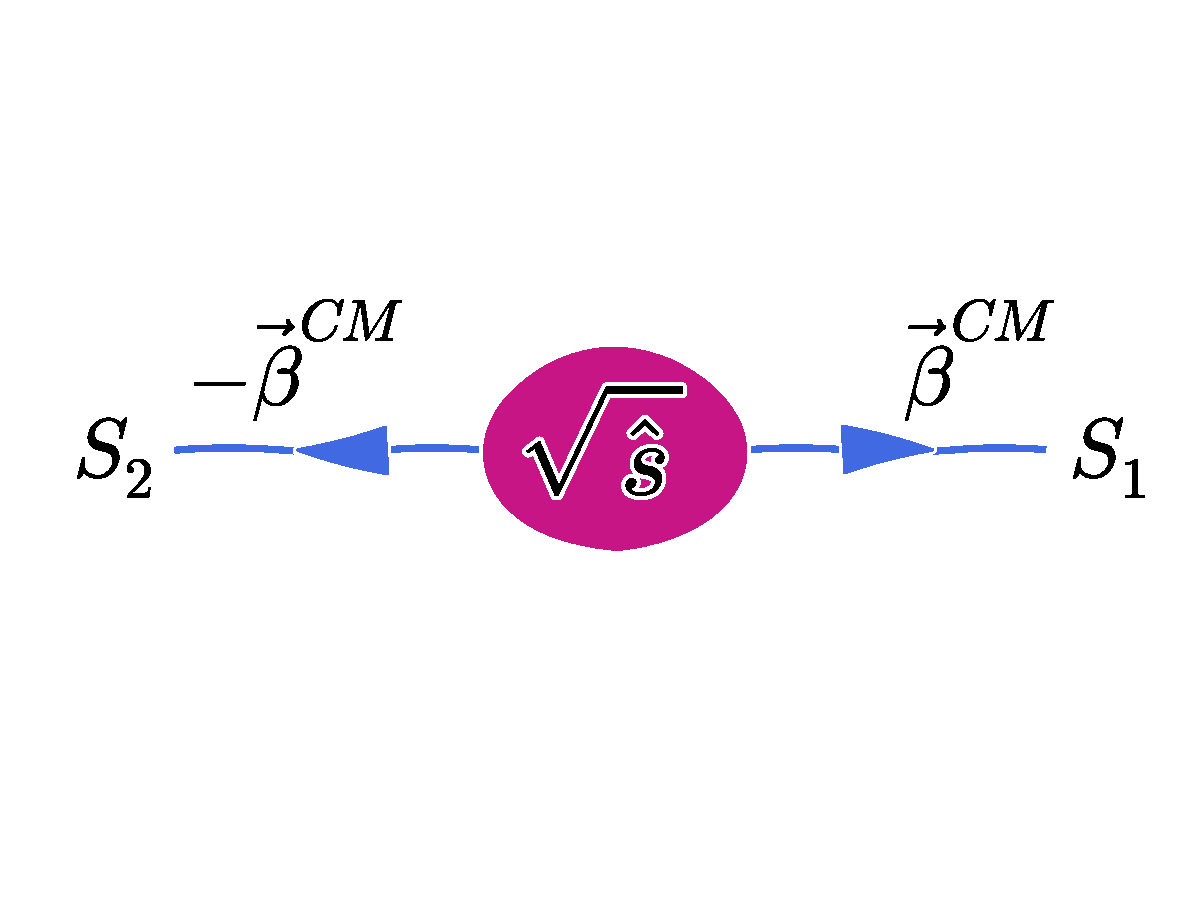
\includegraphics[width=0.6\textwidth,clip=true,trim=0 5.5cm 0
4.5cm]{figures/razor_variables/cm_frame} 
  \caption{Configuration of the center-of-mass frame. The particles $S_1$ and $S_2$ are
produced back to back with velocities $\betaCM$ and $-\betaCM$, respectively. 
\label{fig:razor_CM_frame}}
\end{figure}

To go from the rest frame of $S_1$ ($S_2$) to the CM frame, we need to boost the four-momenta
$q_1^S$ and $\nu_1^S$ ($q_2^S$ and $\nu_2^S$) to the frame travelling at velocity $\betaCM$
($-\betaCM$) with respect to the $S_1$ ($S_2$) rest frame. 
The four-vectors of particles $S_1$ and $S_2$ in the centre-of-mass frame are also obtained by
boosting according to $\betaCM$. They can be written as
\begin{alignat}{6}
  P[S_1] &\equiv s^{\textrm{CM}}_1  &&= \{ E^{\textrm{CM}}_{S_1} , \vec{s}^{\,\textrm{CM}}_{S_1}\} 
&&= M_S \, \gamma^{\textrm{CM}} \, \{ 1 , \betaCM\} , \\ 
  P[S_2] &\equiv s^{\textrm{CM}}_2 &&= \{ E^{\textrm{CM}}_{S_2} , \vec{s}^{\,\textrm{CM}}_{S_2}\}
&&= M_S \, \gamma^{\textrm{CM}} \, \{ 1 , -\betaCM\},  
\end{alignat}
and satisfy the following
\begin{equation}
  (s^{\textrm{CM}}_1 + s^{\textrm{CM}}_1)^2 = \hat{s} = 4 (\gamma^{\textrm{CM}})^2 M_S^2,
\end{equation}
with $\sqrt{\hat{s}}$ the centre-of-mass energy of the collision. 


\paragraph{Lab frame}
The lab frame is the frame where we make our measurements, and is related to the CM frame by a
boost $\vec{\beta}^{\,\textrm{lab}}$. We can decompose this boost into a transverse and longitudinal
part as $\vec{\beta}^{\,\textrm{lab}} = (\vec{\beta}_T,\vec{\beta}_z)$. 
The four-momenta of the $S_i$, $Q_i$ and $\chi_i$ particles are denoted by $s^{\textrm{lab}}_i$,
$q^{\textrm{lab}}_i$, and $\nu^{\textrm{lab}}_i$ respectively. 



\subsection{Derivation of \texorpdfstring{\mr}{MR} \label{sec:razor_mr}}

As mentioned in the previous section, our goal is to express the characteristic scale $M_\Delta$
using lab frame quantities only. Because the problem is kinematically underconstrained, we will
need to make some approximations as we work our way from the lab frame to the $S_i$ rest frame,
reversing the boosts $\vec{\beta}^{\,\textrm{lab}}$ and $\betaCM$ as we go along. 

The models of new physics that we aim to target with the razor variables all predict that the new
particles are heavy. This prediction is the basis of the two approximations we will be making. 

\begin{enumerate}
  \item If $M_S$ is large compared to $\sqrt{s}$, then the particles $S_1$ and $S_2$ will be
produced near the $\sqrt{\hat{s}} = 2 M_S$ threshold. This means that $\gamma^{\textrm{CM}} \approx
1$. We will thus assume that $\gamma^{\textrm{CM}} = 1$, which means that $\betaCM \rightarrow 0$. 
The CM frame is thus equal to both $S_i$ rest frames after this first approximation. 
  \item The transverse boost between lab frame and CM frame can be approximated by 
  \begin{equation}
    |\vec{\beta}_T| \approx \frac{\pt^{\rm ISR}}{\sqrt{\hat{s}}} \lesssim \frac{\pt^{\rm
ISR}}{2M_S},
  \end{equation}
  where $\pt^{\rm ISR}$ is the magnitude of the vectorial sum of the transverse momentum of the
initial state radiation. For large values of $M_S$ we find $\vec{\beta}_T \ll 1$. We thus assume
that $\vec{\beta}_T \rightarrow 0$, and thus $\vec{\beta}^{\,\textrm{lab}} \rightarrow
\vec{\beta}_z$.
\end{enumerate}
The results of these two approximations is that we only need a longitudinal boost $\vec{\beta}_z$
to take us from the lab frame to the approximate $S_i$ rest frames. 
In this so-called \textit{rough-approximation frame}, or \textit{R-frame}, we have that
\begin{alignat}{4}
  |\vec{q}^{\,R}_1|         &= |\vec{q}^{\,R}_2| &&= \frac{M_\Delta}{2} , \\
  \textrm{or } E_{Q_1}^R &= E_{Q_2}^R     &&= \frac{M_\Delta}{2}.
\label{eq:razor_equal_energy_R_frame}
\end{alignat}
cf. Eq.~\ref{eq:razor_equal_momenta}. Using this constraint, we can compute the boost $\beta^R$
that will take us from the lab frame to the R-frame. We start from the basic Lorentz
transformations for energy and momentum, 
\begin{align}
  E_{Q_i}^R      &= \gamma^R \left( E_{Q_i}^{\textrm{lab}} - \beta^R \vec{q}_{iz}^{\,\textrm{lab}}
\right) , \\
  \vec{q}_{iz}^R &= \gamma^R \left( \vec{q}_{iz}^{\,\textrm{lab}} - \beta^R E_{Q_i}^{\textrm{lab}}
\right) .
\end{align}
Using Eq.~\ref{eq:razor_equal_energy_R_frame} we find
\begin{equation}
  E_{Q_1}^{\textrm{lab}} - \beta^R \vec{q}_{1z}^{\,\textrm{lab}} = E_{Q_2}^{\textrm{lab}} - \beta^R
\vec{q}_{2z}^{\,\textrm{lab}} ,
\end{equation}
and thus for the boost $\beta^R$
\begin{equation}
  \beta^R = \frac{E_{Q_1}^{\textrm{lab}} - E_{Q_2}^{\textrm{lab}}}{\vec{q}_{1z}^{\,\textrm{lab}} -
\vec{q}_{2z}^{\,\textrm{lab}}} . \label{eq:razor_beta_R}
\end{equation}
The Lorentz factor $\gamma^R$ can be expressed as
\begin{align}
  \gamma^R &= \frac{1}{\sqrt{1 - (\beta^R)^2}} \\
	   &= \frac{1}{\sqrt{1 - \left( \frac{E_{Q_1}^{\textrm{lab}} -
E_{Q_2}^{\textrm{lab}}}{\vec{q}_{1z}^{\,\textrm{lab}} -
\vec{q}_{2z}^{\,\textrm{lab}}} \right)^2}} \\
           &= \frac{ \vec{q}_{1z}^{\,\textrm{lab}} - \vec{q}_{2z}^{\,\textrm{lab}} }{\sqrt{ \left(
 \vec{q}_{1z}^{\,\textrm{lab}} - \vec{q}_{2z}^{\,\textrm{lab}} \right)^2 - \left(
 E_{Q_1}^{\textrm{lab}} - E_{Q_2}^{\textrm{lab}}\right)^2 }} \label{eq:razor_gamma_R}
\end{align}

We now define \mr as
\begin{equation}
  \mr \equiv 2 |\vec{q}^{\,R}| = M_\Delta .
\end{equation}
It is interesting to note that \mr is invariant under longitudinal boosts. Using
Eq.~\ref{eq:razor_beta_R} and Eq.~\ref{eq:razor_gamma_R}, we can express \mr using lab frame
quantities only. 

\begin{align}
  \mr &= E_{Q_1}^R + E_{Q_2}^R \\
      &= \gamma^R \left( E_{Q_1}^{\textrm{lab}} + E_{Q_2}^{\textrm{lab}} - \beta^R (
\vec{q}_{1z}^{\,\textrm{lab}} + \vec{q}_{2z}^{\,\textrm{lab}}) \right) \\
      &= \frac{\left( \vec{q}_{1z}^{\,\textrm{lab}} - \vec{q}_{2z}^{\,\textrm{lab}}\right) 
               \left( E_{Q_1}^{\textrm{lab}} + E_{Q_2}^{\textrm{lab}} - \frac{E_{Q_1}^{\textrm{lab}}
- E_{Q_2}^{\textrm{lab}}}{\vec{q}_{1z}^{\,\textrm{lab}} - \vec{q}_{2z}^{\,\textrm{lab}}}
(\vec{q}_{1z}^{\,\textrm{lab}} + \vec{q}_{2z}^{\,\textrm{lab}}) \right)}
              { \sqrt{ \left( \vec{q}_{1z}^{\,\textrm{lab}} - \vec{q}_{2z}^{\,\textrm{lab}}
\right)^2 
                      -\left( E_{Q_1}^{\textrm{lab}} - E_{Q_2}^{\textrm{lab}}\right)^2 }} \\
      &= \frac{\left( \vec{q}_{1z}^{\,\textrm{lab}} - \vec{q}_{2z}^{\,\textrm{lab}} \right) 
               \left( E_{Q_1}^{\textrm{lab}} + E_{Q_2}^{\textrm{lab}} \right) 
               - 
               \left( E_{Q_1}^{\textrm{lab}} - E_{Q_2}^{\textrm{lab}} \right)
               \left( \vec{q}_{1z}^{\,\textrm{lab}} + \vec{q}_{2z}^{\,\textrm{lab}} \right) }
              { \sqrt{ \left( \vec{q}_{1z}^{\,\textrm{lab}} - \vec{q}_{2z}^{\,\textrm{lab}}
\right)^2 
                      -\left( E_{Q_1}^{\textrm{lab}} - E_{Q_2}^{\textrm{lab}}\right)^2 }} \\
      &= \frac{2 \left( \vec{q}_{1z}^{\,\textrm{lab}} E_{Q_2}^{\textrm{lab}} 
                       - \vec{q}_{2z}^{\,\textrm{lab}} E_{Q_1}^{\textrm{lab}} \right)}
              { \sqrt{ \left( \vec{q}_{1z}^{\,\textrm{lab}} - \vec{q}_{2z}^{\,\textrm{lab}}
\right)^2 
                      -\left( E_{Q_1}^{\textrm{lab}} - E_{Q_2}^{\textrm{lab}}\right)^2 }}
\end{align}
Our final expression for \mr in lab frame quantities becomes
\begin{equation}
  \mr = 2 \sqrt { \frac{ \left( \vec{q}_{1z}^{\,\textrm{lab}} E_{Q_2}^{\textrm{lab}} 
                       - \vec{q}_{2z}^{\,\textrm{lab}} E_{Q_1}^{\textrm{lab}} \right) ^2}
                       { \left( \vec{q}_{1z}^{\,\textrm{lab}} - \vec{q}_{2z}^{\,\textrm{lab}}
\right)^2 
                        -\left( E_{Q_1}^{\textrm{lab}} - E_{Q_2}^{\textrm{lab}}\right)^2 }} . 
\end{equation}
As the R-frame is only an approximation of the $S_i$ rest frames, \mr will be distributed around
the characteristic scale $M_\Delta$ with degrading resolution as the Lorentz factor increases. 
More generally, the peak value of \mr scales as $\gamma^{\textrm{CM}}M_\Delta$.

We can use \mr as a way to distinguish signal from background, in particular background from QCD
multijet production. Let's consider QCD dijet production. In the dijet rest frame we have for the
four-momenta of the two jets, $k_1$ and $k_2$
\begin{align}
  k_1 &= \frac{\sqrt{\hat{s}}}{2} \{1, \vec{v}\} ,\\
  k_2 &= \frac{\sqrt{\hat{s}}}{2} \{1, -\vec{v}\},
\end{align}
where $\sqrt{\hat{s}}$ is the center-of-mass energy of the partonic subprocess, and $\vec{v}$ is a
unit vector along the dijet axis. For this type of event, $\mr = \sqrt{\hat{s}}$, and is thus
sharply falling. Signal will thus appear as a peak over a falling background. Given the large cross
sections for background processes, and small expected cross sections for signal processes, this
discrimination by itself is not sufficient. There is, however, more information available in the
event. We have yet to use the transverse degrees of freedom. These will be incorporated in \rsq, as
explained in the next section. 

\subsection{Derivation of \texorpdfstring{\rsq}{R2} \label{sec:razor_r2}}

We will now create a second way to estimate $M_\Delta$, utilizing the transverse information in the
event, as encoded in the missing transverse momentum. We start by defining the variable $M_{2S}$
using the four-vectors $q_i^{\textrm{lab}}$ and $\nu_i^{\textrm{lab}}$
\begin{equation}
  M_{2S} = \sqrt{\frac{1}{2} \left[  (q_1^{\textrm{lab}} + \nu_1^{\textrm{lab}})^2 +
(q_2^{\textrm{lab}} + \nu_2^{\textrm{lab}})^2 \right] } . \label{eq:razor_M2S}
\end{equation}
As the sum $q_i^{\textrm{lab}} + \nu_i^{\textrm{lab}}$ is just the four-vector associated with
$S_i$, we immediately see that $M_{2S} = M_S$. Expanding Eq.~\ref{eq:razor_M2S} and using $M_{Q_i}
= 0$, we find
\begin{align}
  M_{2S} &= \sqrt{\frac{1}{2} \left( (q_1^{\textrm{lab}})^2 + 2 q_1^{\textrm{lab}}
\nu_1^{\textrm{lab}} + (\nu_1^{\textrm{lab}})^2 + (q_2^{\textrm{lab}})^2 + 2 q_2^{\textrm{lab}}
\nu_2^{\textrm{lab}} + (\nu_2^{\textrm{lab}})^2\right) } \\
         &= \sqrt{ q_1^{\textrm{lab}}\nu_1^{\textrm{lab}} + q_2^{\textrm{lab}}\nu_2^{\textrm{lab}}
+ M_\chi^2} \\
         &= \sqrt{ E^{\textrm{lab}}_{Q_1} E^{\textrm{lab}}_{\nu_1} - \vec{q}^{\,\textrm{lab}}_{1T}
\cdot \vec{\nu}^{\,\textrm{lab}}_{1T} - \vec{q}^{\,\textrm{lab}}_{1z} \cdot
\vec{\nu}^{\,\textrm{lab}}_{1z}
                  + E^{\textrm{lab}}_{Q_2} E^{\textrm{lab}}_{\nu_2} - \vec{q}^{\,\textrm{lab}}_{2T}
\cdot \vec{\nu}^{\,\textrm{lab}}_{2T} - \vec{q}^{\,\textrm{lab}}_{2z} \cdot
\vec{\nu}^{\,\textrm{lab}}_{2z} + M_\chi^2} .
\end{align}
Unfortunately we do not a priori know the mass of the $\chi_i$ particles. We will choose $M_\chi =
0$. As a result $M_{2S}$ will now give us a distribution, with endpoint at $M_S$. For the
particular case $M_\chi = 0$, we actually have $M_S = \frac{M_S^2-M_\chi^2}{M_S} = M_\Delta$.
Consequently, the endpoint of $M_{2S}$ gives us a second way to access the characteristic scale
$M_\Delta$.

The $\chi_i$ particles are assumed to be only weakly interacting. They pass through the detector
unseen. When we make the balance of momentum for each event, we can thus infer the existence of
these particles. At a hadron collider we can only make this balance in the transverse plane. The
transverse component of $M_{2S}$ is given by
\begin{equation}
  (M_{2S})_T = \sqrt{ |\vec{q}^{\,\textrm{lab}}_{1T}| |\vec{\nu}^{\,\textrm{lab}}_{1T}| -
\vec{q}^{\,\textrm{lab}}_{1T} \cdot \vec{\nu}^{\,\textrm{lab}}_{1T} 
                  + |\vec{q}^{\,\textrm{lab}}_{2T}| |\vec{\nu}^{\,\textrm{lab}}_{2T}| -
\vec{q}^{\,\textrm{lab}}_{2T} \cdot \vec{\nu}^{\,\textrm{lab}}_{2T}} ,
\end{equation}
where we have used the assumptions that both $Q_i$ and $\chi_i$ are massless. 
In the considered signal topology we have two unseen particles, $\chi_1$ and $\chi_2$.
Experimentally we can only access the sum of their transverse momenta, which in absence of detector
effects is given by the missing transverse momentum \VEtmiss. Making the assumption that the
\VEtmiss is divided equally among both $\chi_i$ particles, we find
\begin{equation}
  \mtr = \sqrt{\frac{|\VEtmiss|}{2} \left(|\vec{q}^{\,\textrm{lab}}_{1T}| +
|\vec{q}^{\,\textrm{lab}}_{2T}| \right) - \frac{\VEtmiss}{2} \cdot
\left(\vec{q}^{\,\textrm{lab}}_{1T} + \vec{q}^{\,\textrm{lab}}_{2T} \right)} .
\end{equation}

We now define the dimensionless variable $\mathrm{R}$ as
\begin{equation}
  \mathrm{R} \equiv \frac{\mtr}{\mr} .
\end{equation}
This variable peaks at around 0.5 for signal events, since it is the ratio of two variables that
estimate the same scale, with an additional geometric factor to take into account that
$\mathrm{M_T^R}$ only contains transverse information. For QCD dijet events $\mathrm{R}$ equals 0
for an ideal detector. Placing a minimum requirement on this variable can thus
be effectively used to suppress background events.


\subsection{Improved \texorpdfstring{\mr and \rsq}{MR and R2} definitions
\label{sec:razor_mr_r2_improved}}

The razor frame as defined in the previous section has a number of useful features, such as \mr
being invariant under longitudinal boosts. It also has one important issue which can occur if the
approximation $\gamma^{\textrm{CM}} = 1$ breaks down. The issue is visible from the expression of
$\beta^R$ in Eq.~\ref{eq:razor_beta_R}. Looking at that equation, we see that it is possible to get
a situation where $|\beta^R| \geq 1$. The boost is then unphysical, and the razor frame ill-defined.
We can remedy this issue by not neglecting $\vec{\beta}_T$, the transverse component of
$\betaCM$. 

% TODO Add the full computation

We again start by making a longitudinal boost $\beta^{L^*}$ from the lab frame. Then we apply a
transverse boost $\vec{\beta}_T^{\,\mathrm{R}^*}$. This boost is applied in opposite directions to
the
decay products of $S_1$ and $S_2$. The two resulting frames are called $\mathrm{R}^*$-frames, and
have to satisfy the requirement that the magnitude of the momenta of $Q_1$ and $Q_2$ in their
respective $\mathrm{R^*}$-frame are equal. 

This constraint can be rewritten as
\begin{equation}
  \gamma^{L^*} (E_{Q_1}^{\textrm{lab}} - E_{Q_2}^{\textrm{lab}}) - \gamma^{L^*} \beta^{L^*}
(q_{1z}^{\textrm{lab}} - q_{2z}^{\textrm{lab}}) = \vec{\beta}_T^{R^*} \cdot
(\vec{q}_{1T}^{\,\textrm{lab}} + \vec{q}_{2T}^{\,\textrm{lab}}), 
\end{equation}
where we have used the Lorentz transformations for energy corresponding to the two consecutive
boosts,
\begin{align}
  E_{Q_i}^{L^*} &= \gamma^{L^*} (E_{Q_i}^{\textrm{lab}} - \beta^{L^*} q_{iz}^{\textrm{lab}} ) , \\
  E_{Q_1}^{R^*} &= \gamma_T^{R^*} (E_{Q_1}^{L^*} - \vec{\beta}_T^{\,R^*} \cdot
\vec{q}_{1T}^{\,\textrm{lab}}) , \\
  E_{Q_2}^{R^*} &= \gamma_T^{R^*} (E_{Q_2}^{L^*} + \vec{\beta}_T^{\,R^*} \cdot
\vec{q}_{2T}^{\,\textrm{lab}}) .
\end{align}
Introducing the unit vector $\hat{\beta}_T^{\mathrm{R}^*}$ such that $\vec{\beta}_T^{\mathrm{R}^*} =
\beta_T^{\mathrm{R}^*} \hat{\beta}_T^{\mathrm{R}^*}$, we find for the magnitude of the transverse
boost
\begin{equation}
  \beta_T^{\mathrm{R}^*} = \frac{\gamma^{L^*} (E_{Q_1}^{\textrm{lab}} - E_{Q_2}^{\textrm{lab}}) -
\gamma^{L^*} \beta^{L^*} (q_{1z}^{\textrm{lab}} - q_{2z}^{\textrm{lab}})}{\hat{\beta}_T^{R^*} \cdot
(\vec{q}_{1T}^{\,\textrm{lab}} + \vec{q}_{2T}^{\,\textrm{lab}})}
\end{equation}

In analogy with our previous discussion we define the $\mathrm{R}^*$-frame mass $\mathrm{M_{R^*}}$
as
\begin{align}
  \mathrm{M_{R^*}} &\equiv 2 |\vec{q}_1^{\,\mathrm{R}^*}| = 2 |\vec{q}_2^{\,\mathrm{R}^*}| \\
                  &= \frac{2\gamma^{L^*} \hat{\beta}_T^{\mathrm{R}^*} \cdot \left[
(E_{Q_1}^{\textrm{lab}}\vec{q}_{2T}^{\,\textrm{lab}} +
E_{Q_2}^{\textrm{lab}}\vec{q}_{1T}^{\,\textrm{lab}}) - \beta^{L^*}
(q_{1z}^{\textrm{lab}}\vec{q}_{2T}^{\,\textrm{lab}} +
q_{2z}^{\textrm{lab}}\vec{q}_{1T}^{\,\textrm{lab}}) \right]}
                           {\sqrt{|\hat{\beta}_T^{R^*} \cdot (\vec{q}_{1T}^{\,\textrm{lab}} +
\vec{q}_{2T}^{\,\textrm{lab}})|^2 - (\gamma^{L^*})^2 \left[ E_{Q_1}^{\textrm{lab}} -
E_{Q_2}^{\textrm{lab}} - \beta^{L^*} (q_{1z}^{\textrm{lab}} - q_{2z}^{\textrm{lab}}) \right]^2}}
\end{align}

To fully compute $\mathrm{M_{R^*}}$ we need to pick a value for $\beta_T^{\mathrm{R}^*}$ and
$\beta^{L^*}$. The configurations that led to unphysical \mr values have the property that the
momenta of $Q_1$ and $Q_2$ point in the same direction in the transverse plane, with $\betaCM$
pointing in the same or the opposite direction. Based on this observation, we choose a direction
for $\hat{\beta}_T^{\mathrm{R}^*}$ that maximizes $|\hat{\beta}_T^{R^*} \cdot
(\vec{q}_{1T}^{\,\textrm{lab}} + \vec{q}_{2T}^{\,\textrm{lab}})|$. The direction that maximizes this
quantity is aligned with the direction of $\vec{q}_{1T}^{\,\textrm{lab}} +
\vec{q}_{2T}^{\,\textrm{lab}}$. Realizing that a unit vector can be expressed as a vector indicating
the direction divided by the norm of that vector, we find for $\hat{\beta}_T^{\mathrm{R}^*}$ 
\begin{equation}
  \hat{\beta}_T^{\mathrm{R}^*} = \frac{\vec{q}_{1T}^{\,\textrm{lab}} +
\vec{q}_{2T}^{\,\textrm{lab}}}{|\vec{q}_{1T}^{\,\textrm{lab}} + \vec{q}_{2T}^{\textrm{lab}}|}
\label{eq:razor_beta_T_Rstar}
\end{equation}
We still want $\mathrm{M_{R^*}}$ to be invariant under longitudinal boosts. Therefore we choose
$\beta^{L^*}$ according to the condition $\frac{\partial \mathrm{M_{R^*}}}{\partial \beta^{L^*}} =
0$.
We find
\begin{equation}
  \beta^{L^*} = \frac{q_{1z}^{\textrm{lab}} + q_{2z}^{\textrm{lab}}}
{E_{Q_1}^{\textrm{lab}} + E_{Q_2}^{\textrm{lab}}}
\label{eq:razor_beta_Lstar}
\end{equation}

Substituting Eq.~\ref{eq:razor_beta_T_Rstar} and Eq.~\ref{eq:razor_beta_Lstar} in the expression for
$\mathrm{M_{R^*}}$ we find
\begin{equation}
  \mathrm{M_{R^*}} = \sqrt{\left( E_{Q_1}^{\textrm{lab}} + E_{Q_2}^{\textrm{lab}}\right)^2 
                        - \left( q_{1z}^{\textrm{lab}} + q_{2z}^{\textrm{lab}} \right)^2 
                        - \frac{(|\vec{q}_{1T}^{\,\textrm{lab}}|^2 -
|\vec{q}_{2T}^{\,\textrm{lab}}|^2 )^2}{|\vec{q}_{1T}^{\,\textrm{lab}} +
\vec{q}_{2T}^{\,\textrm{lab}}|^2} } .
\end{equation}
We can also express $\gamma_T^{R^*}$ in lab frame observables,
\begin{equation}
  \gamma_T^{R^*} = \sqrt{ \frac{\left( E_{Q_1}^{\textrm{lab}} + E_{Q_2}^{\textrm{lab}}\right)^2 
                        - \left( q_{1z}^{\textrm{lab}} + q_{2z}^{\textrm{lab}} \right)^2 }
                              {\left( E_{Q_1}^{\textrm{lab}} + E_{Q_2}^{\textrm{lab}}\right)^2 
                        - \left( q_{1z}^{\textrm{lab}} + q_{2z}^{\textrm{lab}} \right)^2 
                        - \frac{(|\vec{q}_{1T}^{\textrm{lab}}|^2 -
|\vec{q}_{2T}^{\,\textrm{lab}}|^2 )^2}{|\vec{q}_{1T}^{\,\textrm{lab}} +
\vec{q}_{2T}^{\,\textrm{lab}}|^2}}} . 
\end{equation}
The peak value of the $\mathrm{M_{R^*}}$ distribution is at $M_\Delta$, whereas the peak value for
$\gamma_T^{R*}\mathrm{M_{R*}}$ is at $\gamma^{\textrm{CM}}M_\Delta$, as was the case for \mr
earlier. This motivates us to redefine \mr as
\begin{equation}
  \mr = \gamma_T^{R^*}\mathrm{M_{R^*}} = \sqrt{\left( E_{Q_1}^{\textrm{lab}} +
E_{Q_2}^{\textrm{lab}}\right)^2 - \left( q_{1z}^{\textrm{lab}} +
q_{2z}^{\textrm{lab}} \right)^2} ,
\end{equation}
which is still longitudinally invariant, but does not suffer from unphysical boosts.
The definition of \mtr remains the same, and $\mathrm{R} = \frac{\mtr}{\mr}$ is now defined using
the updated \mr definition.

\textcolor{red}{If there is time, I will try to work through the full derivation.}

\subsection{Generalization to longer decay chains \label{sec:razor_megajet_algorithm}}

In the previous discussion we have always assumed that the new particles decay according to a
two-body decay chain. We can of course envision many other scenarios in which this is no longer the
case. One could have three- or four-body decays, or long decay chains. All of those cases would
result in more than two visible particles in the final state. 

In order to use the same razor formalism, we simply need to cluster all the particles in the event
into two so-called \textit{megajets}. Among all possible clusterings of particles in two groups, we
choose the clustering that minimizes the quadratic sum of invariant masses of the two megajets. The
four-momenta of the megajets, which are used to compute the invariant masses, are defined as the sum
of the four-momenta of their constituents. \mr and \rsq are then defined as before, using the
megajets as the two visible components. 

This approach groups particles travelling in the same direction, and is effective at grouping the
decay products of each of the two initially produced particles. 


\subsection{The razor variables in the razor boost analysis}

As the name already indicates, the razor boost analysis uses the razor variables as the main
discriminating variables. They are well suited for the purpose of the analysis; they are
designed to describe a signal due to pair production of heavy particles, each of which decays to a
massless visible particle and a massive invisible particle, as is the case for the targeted models
in the razor boost analysis. The signal will appear as a peak on an exponentially falling
background. 

For clarity we repeat the \mr and \rsq definitions here, replacing the relevant variables with their
megajet counterparts, with indices ${\rm j}_i$, 
\begin{align}
  \mr &= \sqrt{\left( E_{{\rm j}_1} + E_{{\rm j}_2}\right)^2 - \left( p_{z}^{{\rm j}_1} +
p_{z}^{{\rm j}_2} \right)^2} ,\\
  \rsq &= \frac{\mtr}{\mr} ,\\
  \textrm{with } \mtr &= \sqrt{\frac{|\VEtmiss|}{2} \left(\pt^{{\rm j}_1} + \pt^{{\rm j}_2}
\right) - \frac{\VEtmiss}{2} \cdot \left(\ptvec^{\,{\rm j}_1} + \ptvec^{\,{\rm j}_2}
\right)} ,
\end{align}
where we have defined $\pt$ as the magnitude of the transverse momentum vector $\ptvec$. 

The two-dimensional (2D) distributions of \rsq versus \mr for both background and an example signal
model are shown in Fig.~\ref{fig:razor_MR_Rsq_bg_signal}. A very loose selection is applied,
requiring the presence of a good primary vertex and at least three jets, one of which should have
$\pt > 200$ \GeV. It is clear that the background, dominated by QCD multijet production, is located
in the low \mr and low \rsq regions, and falls off steeply when \mr or \rsq is increased. The
signal, on the other hand, shows a peaking behaviour in \mr and is located substantially higher in
the (\mr,\rsq) space. 
The $\mr$ distribution peaks at higher values for larger sparticle masses and higher mass
differences between the gluino and the LSP. This is illustrated
in Figs.~\ref{fig:razor_MR_R2_T1ttcc} and \ref{fig:razor_MR_R2_T1t1t}, which show the $\mr$ and
$\rsq$ distributions for several signal points using the same loose selection as defined above.
The width of the $\mr$ distribution also increases with the gluino mass. This is why we use an
increasingly larger bin width for $\mr$ when defining our analysis regions. 


\begin{figure}[htpb]
\centering
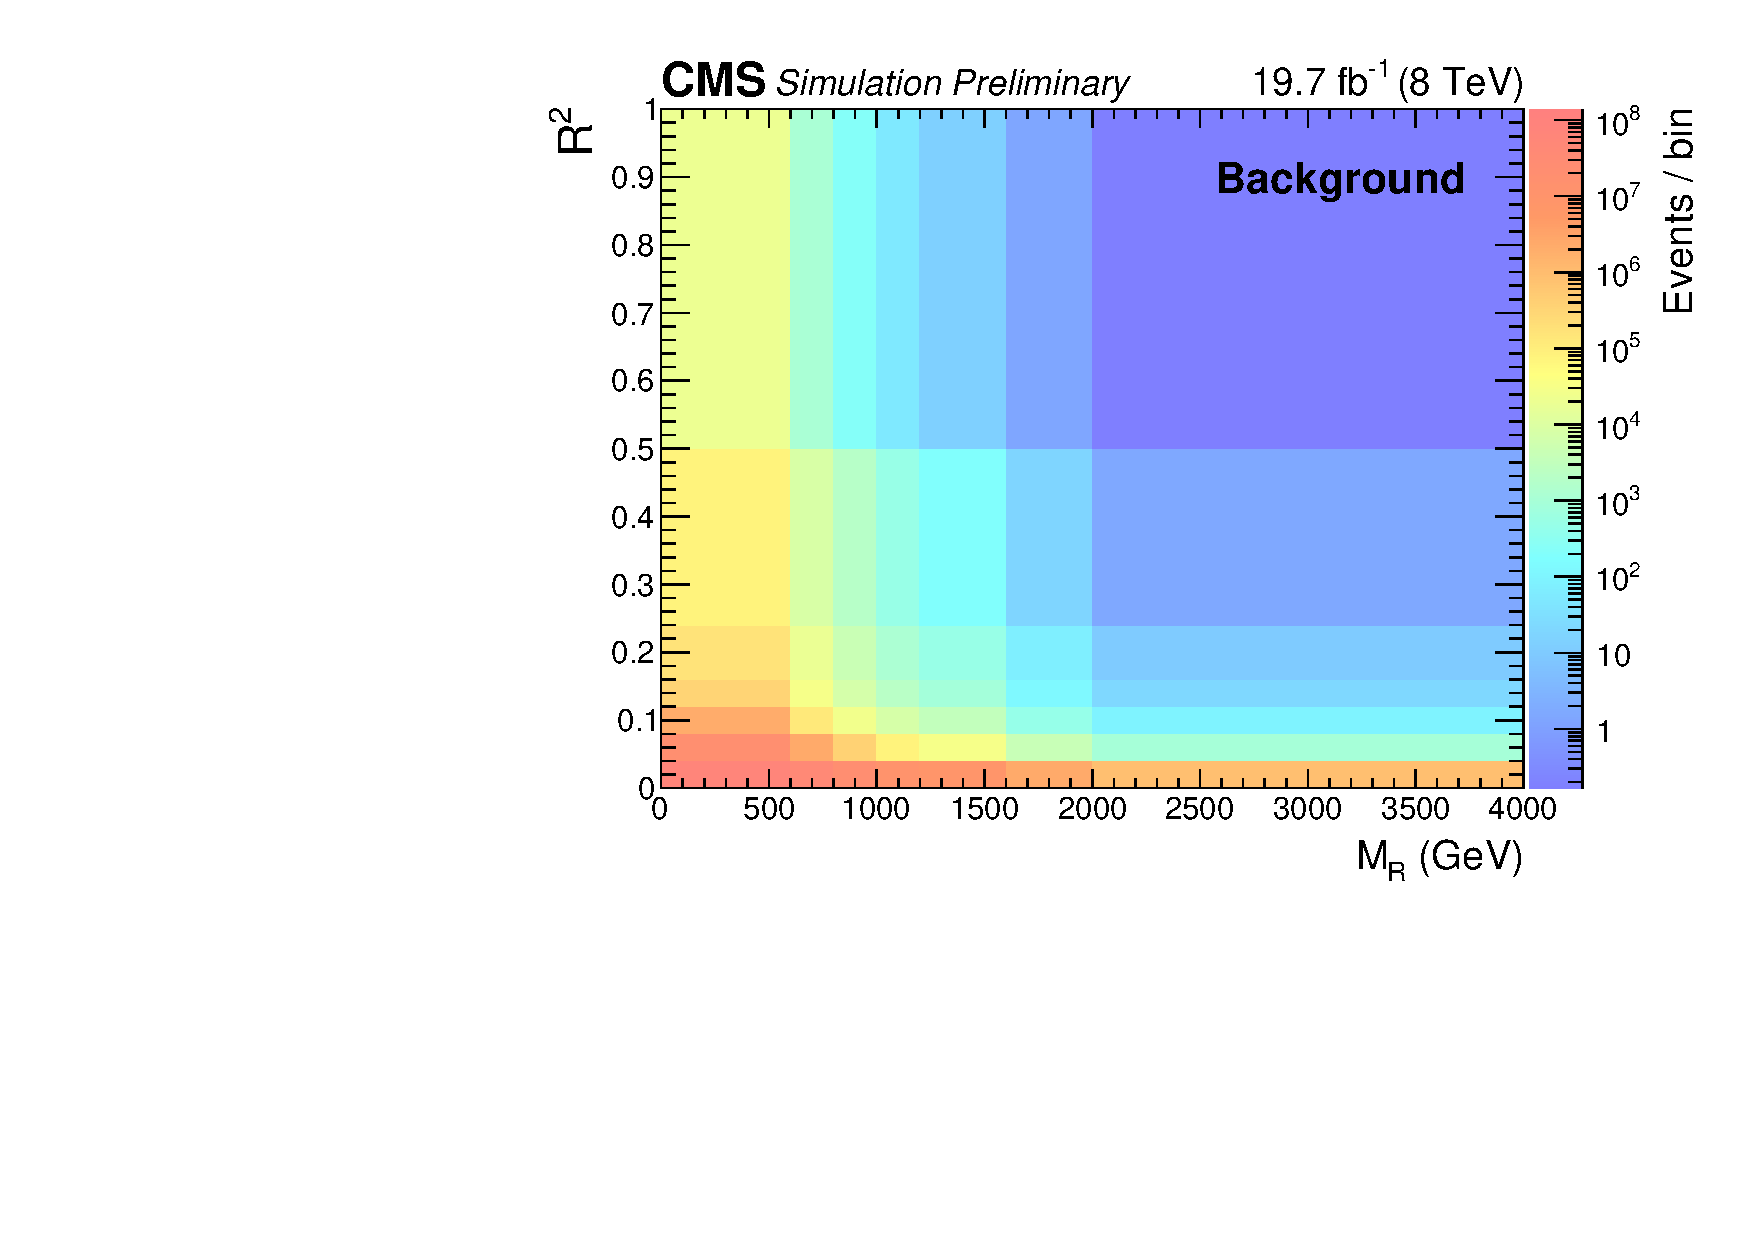
\includegraphics[width=0.49\textwidth]{figures/razor_variables/MR_R2_jet1ptg200_bg} 
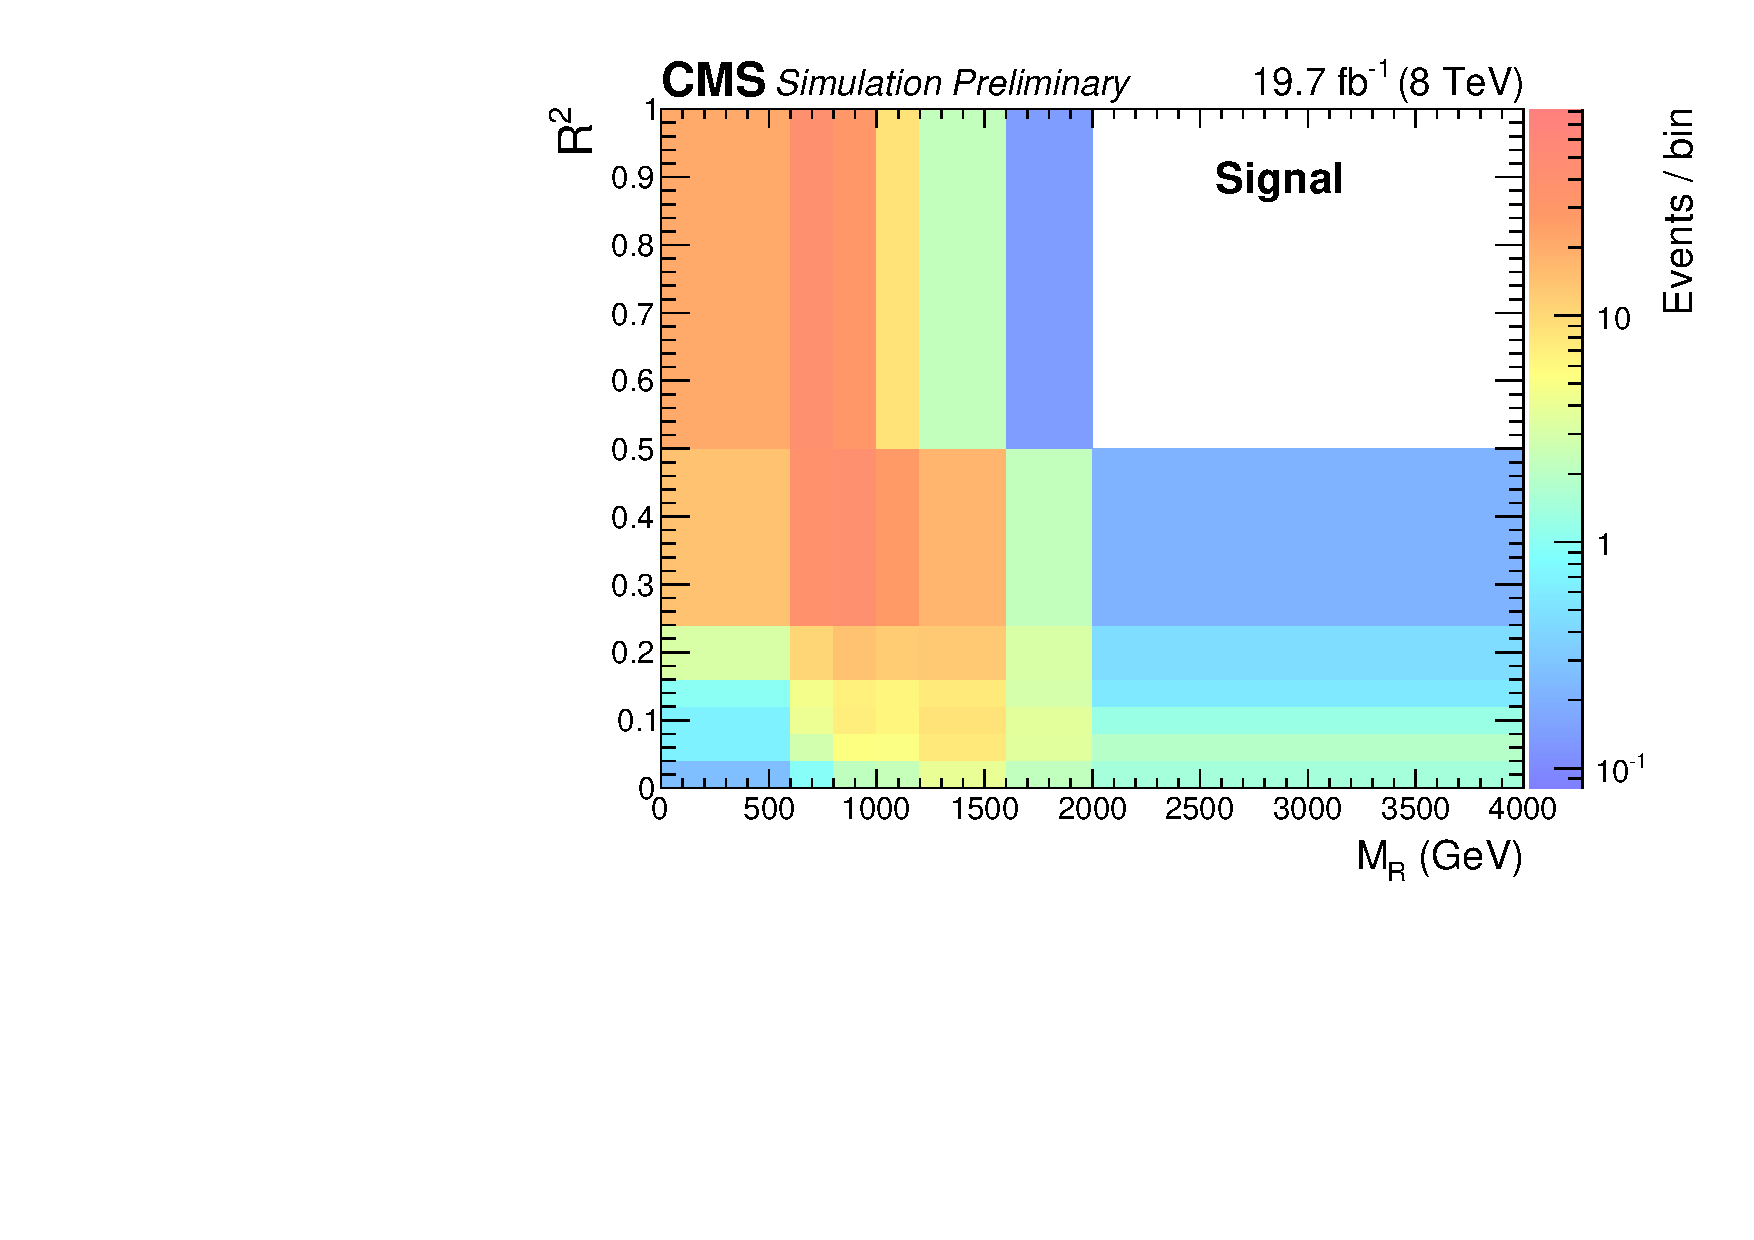
\includegraphics[width=0.49\textwidth]{figures/razor_variables/MR_R2_jet1ptg200_sig}
\caption{Distribution of the overall SM backgrounds and a T1ttcc signal with $m_{\tilde{g}} \,{=}\,
1\TeV$, $m_{\tilde{t}} \,{=}\, 325\GeV$ and $m_{\tilde{\chi}_1^0} \,{=}\, 300\GeV$, both obtained
from MC, on the (\mr,\rsq) space. A very loose selection is used:  a good primary vertex and at
least three jets, one of which should have $\pt > 200$ \GeV. 
\label{fig:razor_MR_Rsq_bg_signal}}
\end{figure}

\begin{figure}[htpb]
\centering
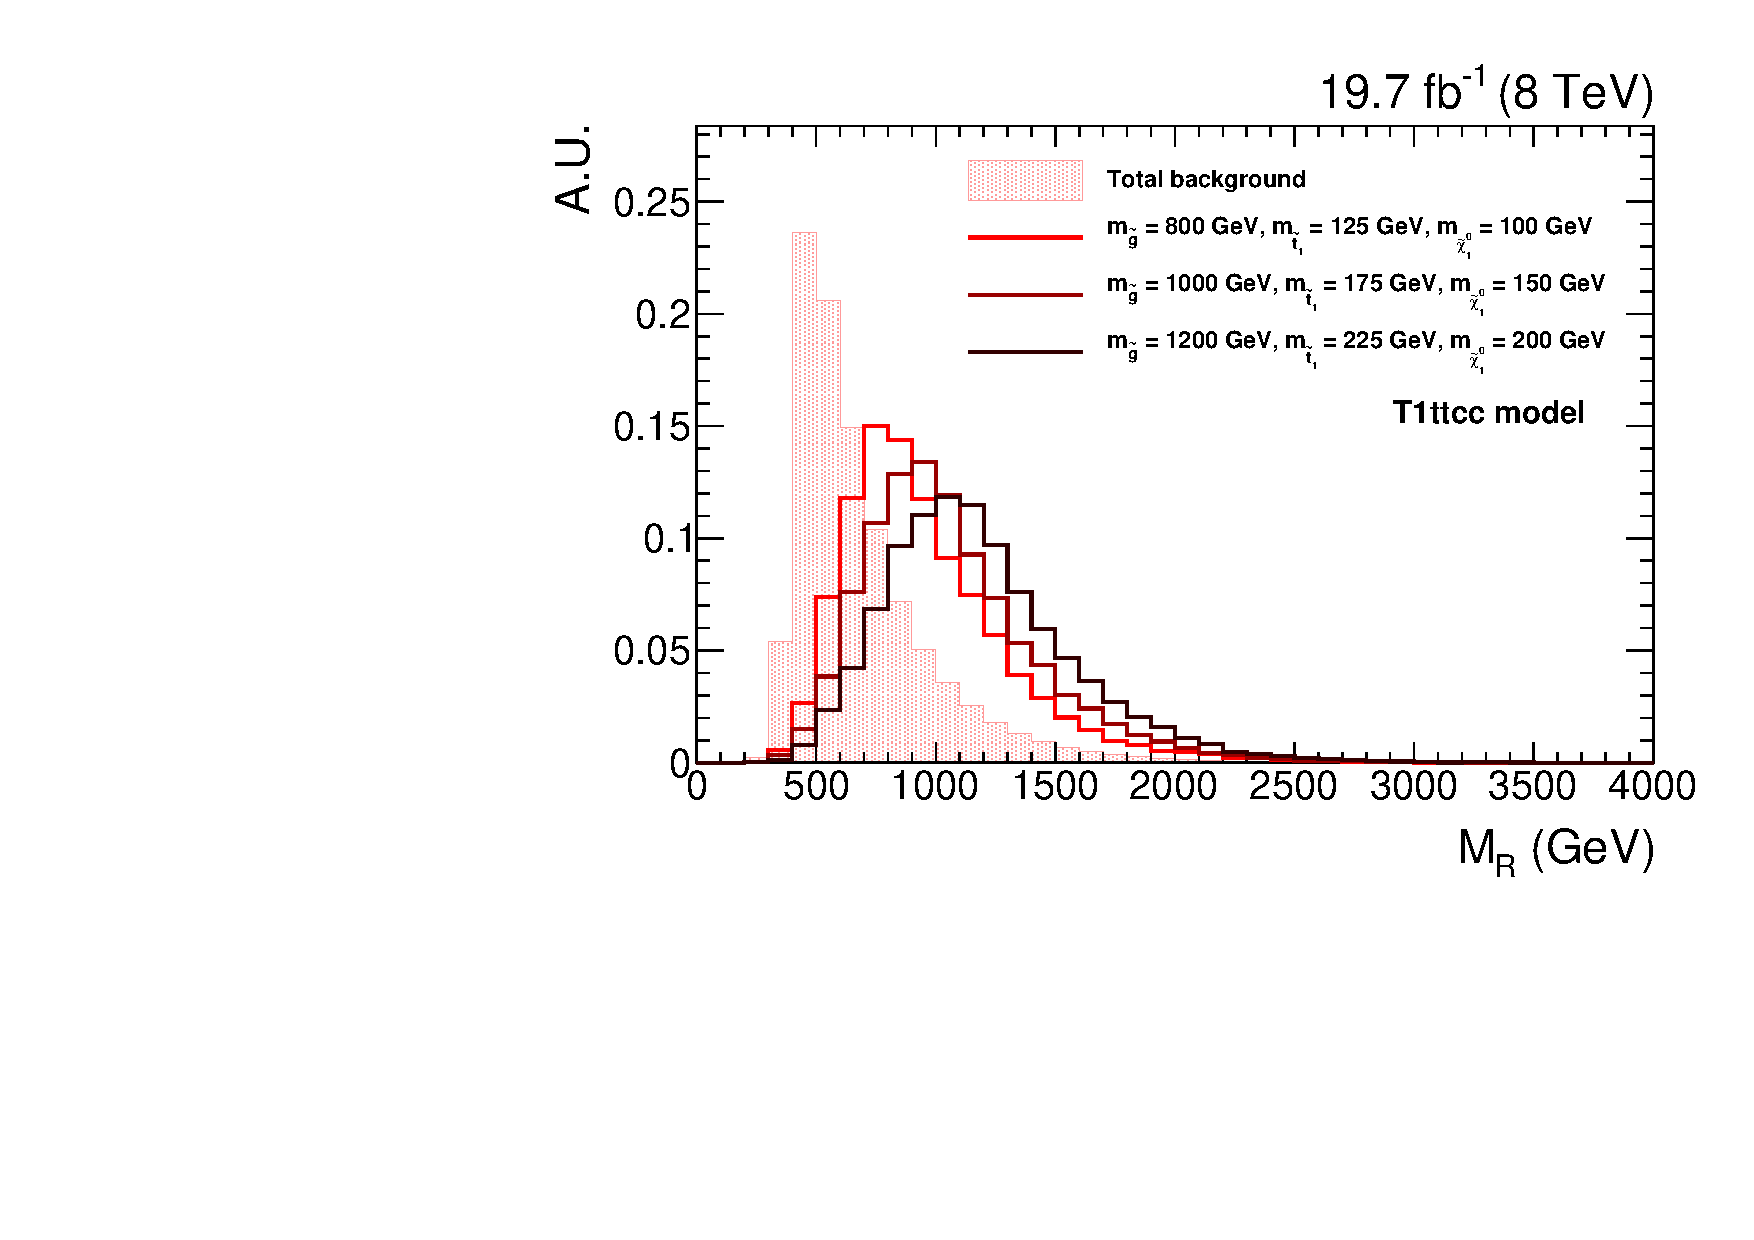
\includegraphics[width=0.48\textwidth]{figures/razor_variables/T1ttcc_MR_comparison} 
~
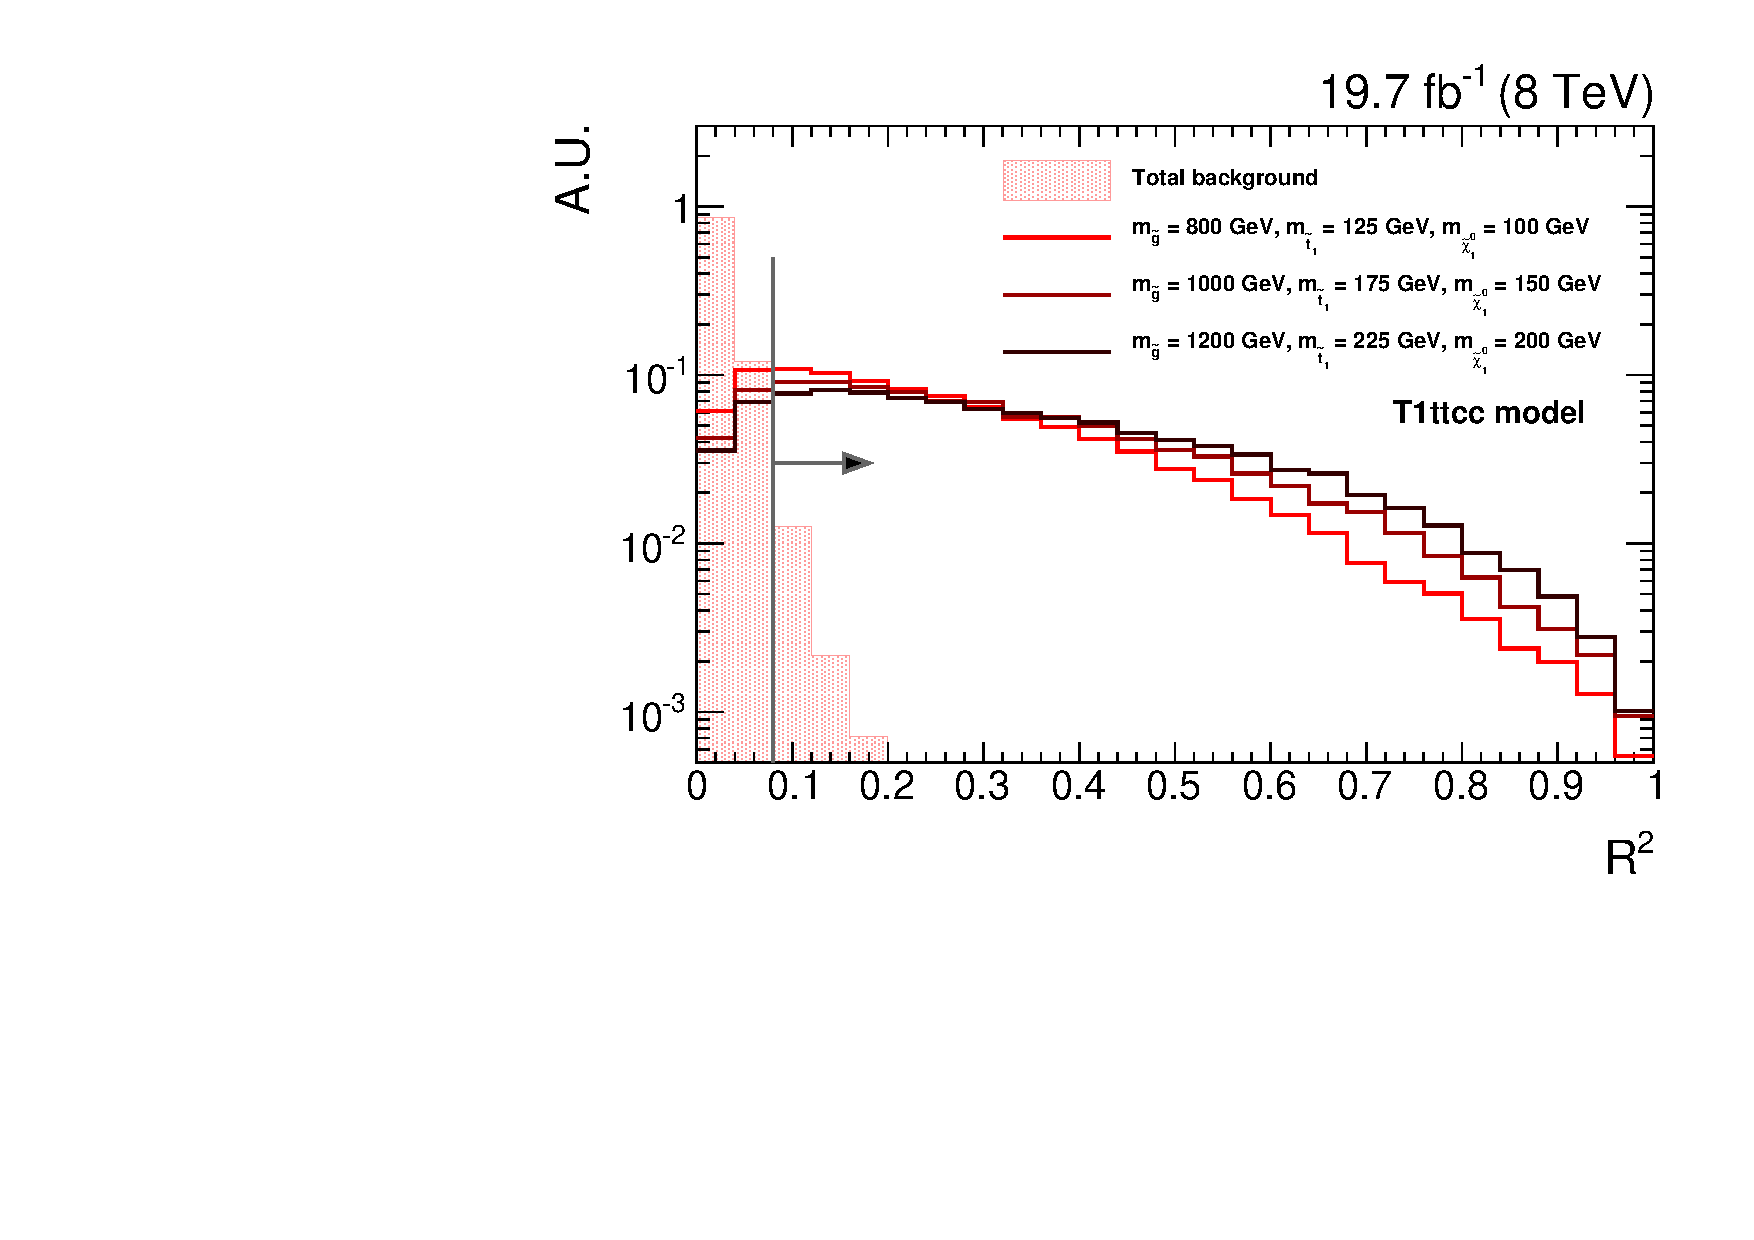
\includegraphics[width=0.48\textwidth]{figures/razor_variables/T1ttcc_R2_comparison}
\caption{Distribution of $\mr$ (left) and $\rsq$ (right) for the total SM background, and several
T1ttcc signal points. A very loose selection is used, including only the requirement of having a
good primary vertex and at least three jets, one of which with $\pt > 200$ \GeV. 
\label{fig:razor_MR_R2_T1ttcc}}
\end{figure}

\begin{figure}[htpb]
\centering
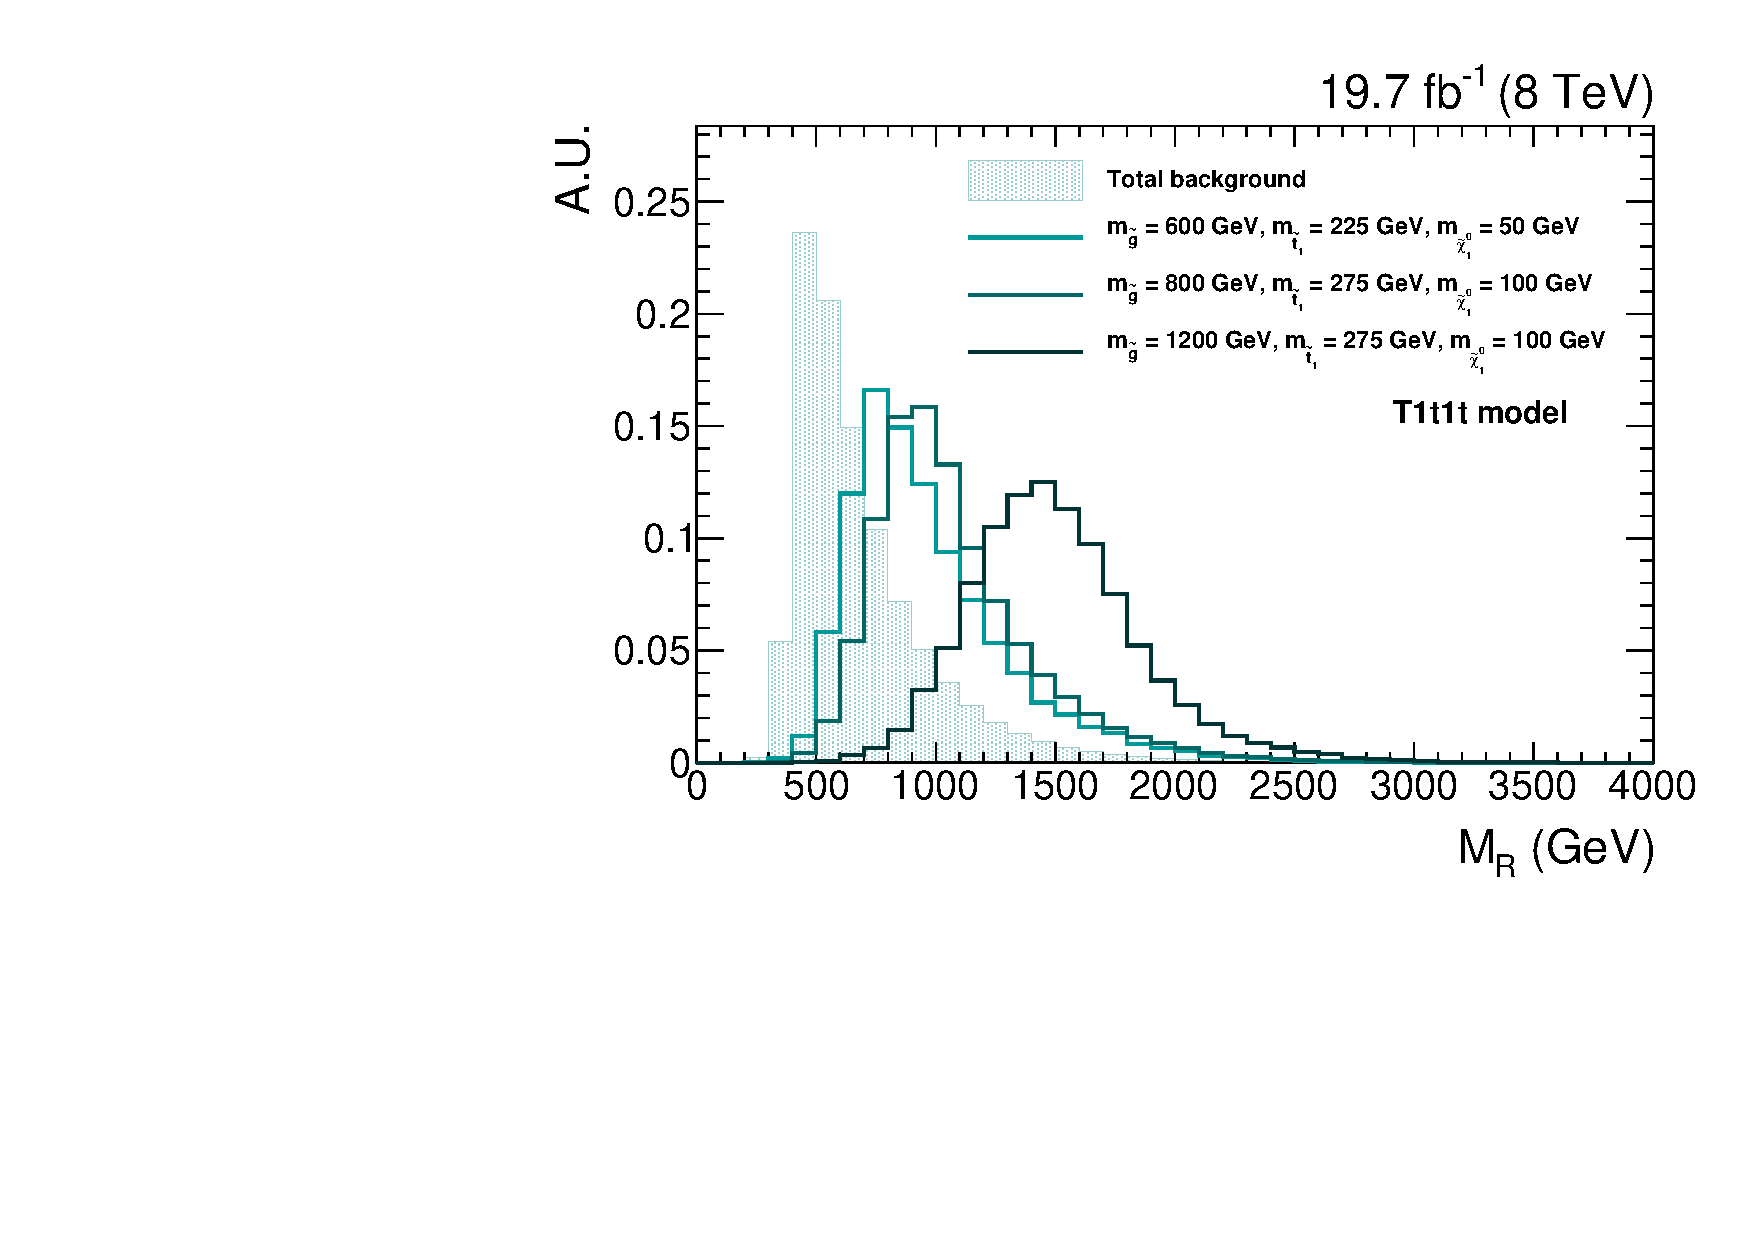
\includegraphics[width=0.48\textwidth]{figures/razor_variables/T1t1t_MR_comparison} 
~
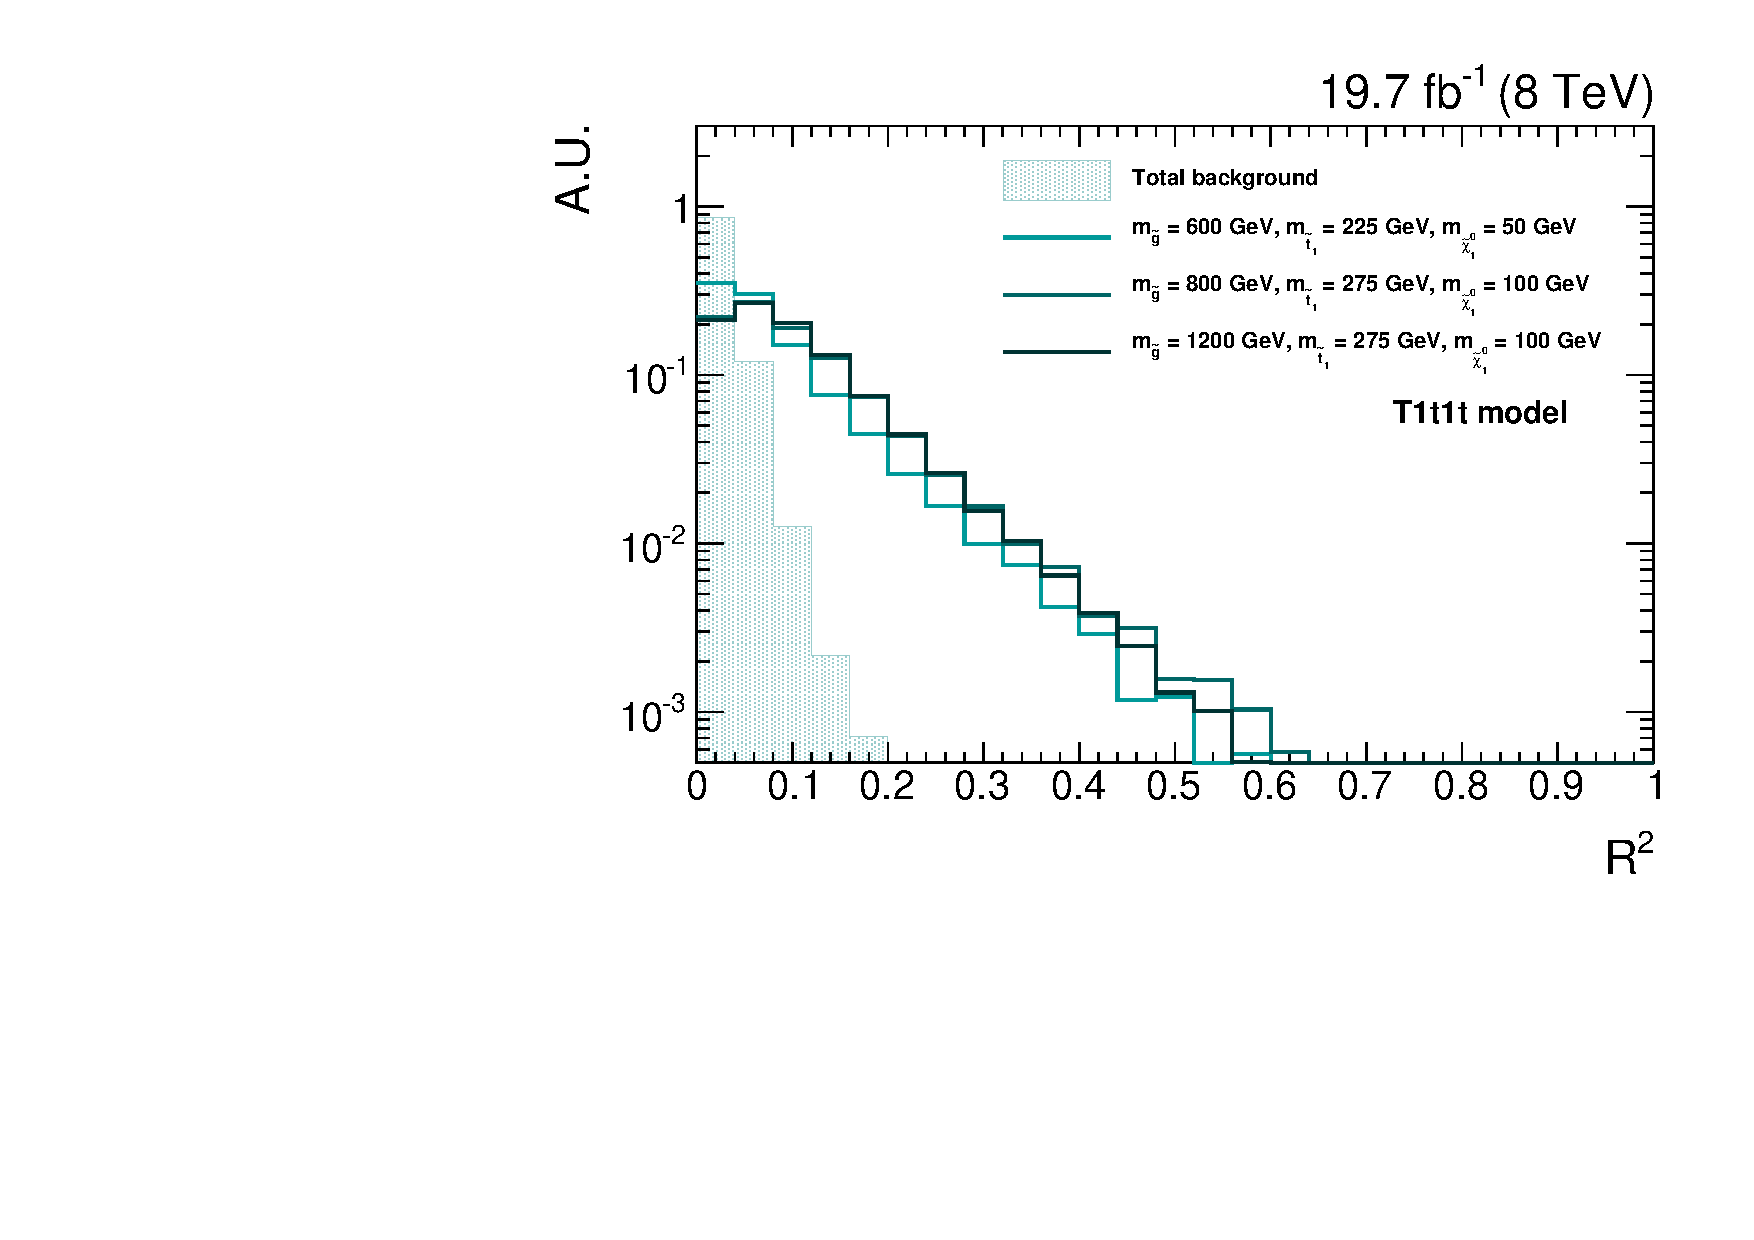
\includegraphics[width=0.48\textwidth]{figures/razor_variables/T1t1t_R2_comparison}
\caption{Distribution of $\mr$ (left) and $\rsq$ (right) for the total SM background, and several
T1t1t signal points. A very loose selection is used, including only the requirement of having a good
primary vertex and at least three jets, one of which with $\pt > 200$ \GeV. 
\label{fig:razor_MR_R2_T1t1t}}
\end{figure}

In order to retain sensitivity to low \ETm scenarios, we choose to reduce the minimal $\rsq$
requirement compared to previous razor
analyses~\cite{Chatrchyan:2011ek,razorPRL,Chatrchyan:2014goa}, while simultaneously raising
the $\mr$ requirement to access the boosted phase space, and keep the background to a
manageable level.
As explained before, $\mr$ is a measure of mass difference, and since high boost requires high mass
differences, we opt to work in the high $\mr$ region to obtain better expected signal
significance. 
The baseline requirement implemented in this analysis is that events fall within the ranges 
\begin{itemize}
\item $\mr > 800\GeV$, 
\item $\rsq > 0.08$.
\end{itemize}
This provides a good balance between background suppression and signal acceptance. 
